
\documentclass[11pt]{exam} % https://www.ctan.org/pkg/exam?lang=en

\usepackage[lmargin=1.in,rmargin=1.in,tmargin=1.in,bmargin=1in]{geometry}
\usepackage{setspace}
\usepackage[pdftex]{graphicx}
\usepackage{titling}
\usepackage[
	pdfauthor={Brian Weinstein},
	pdftitle={Homework 1},
	bookmarks=true,
	colorlinks=true,
	linkcolor=blue,
	urlcolor=blue,
	citecolor=blue,
	pdftex,
	linktocpage=true
	]{hyperref}
\usepackage[textsize=tiny]{todonotes}
\usepackage{float}
\setlength\parindent{0pt}
\usepackage{lipsum}
\usepackage{amsmath}
\usepackage{caption}


\qformat{\textbf{Problem \thequestion: \thequestiontitle}\quad \hfill}


\pagestyle{headandfoot}
\runningheadrule
\firstpageheader{}{}{}
\runningheader{\theauthor}{\thetitle}{\thedate}
\firstpagefooter{}{\thepage}{}
\runningfooter{}{\thepage}{}


\usepackage{xcolor}
\usepackage{adjustbox}
\usepackage{verbatim}
\definecolor{shadecolor}{rgb}{.9, .9, .9}

\newenvironment{code}%
   {\par\noindent\adjustbox{margin=1ex,bgcolor=shadecolor,margin=0ex \medskipamount}\bgroup\minipage\linewidth\verbatim}%
   {\endverbatim\endminipage\egroup}

\newenvironment{codeSmall}%
   {\par\noindent\adjustbox{margin=1ex,bgcolor=shadecolor,margin=0ex \medskipamount}\bgroup\minipage\linewidth\verbatim\footnotesize}%
   {\endverbatim\endminipage\egroup}

\newcommand{\ramsey}{\href{http://www.statisticalsleuth.com/}{Ramsey }}



\begin{document}


\title{STAT W4201 001, Homework 6}
\author{Brian Weinstein (bmw2148)}
\date{Mar 9, 2016}
\maketitle

Code is attached here and also posted at \href{https://github.com/BrianWeinstein/advanced-data-analysis}{https://github.com/BrianWeinstein/advanced-data-analysis}. Where relevant, code snippets and output are are included in-line.

\begin{questions}


\titledquestion{\ramsey 9.14}

\begin{parts}

\part \textit{Draw a matrix of scatterplots of the four variables. Construct it so that the bottom row of plots all have heart on the vertical axis. If you do not have this facility, draw scatterplots of heart versus each of the other variables individually.}

A matrix of pairwise scatterplots is shown in Figure \ref{fig:1a}.

\begin{figure}[!h]
	\centering
	\captionsetup{width=0.8\textwidth}
	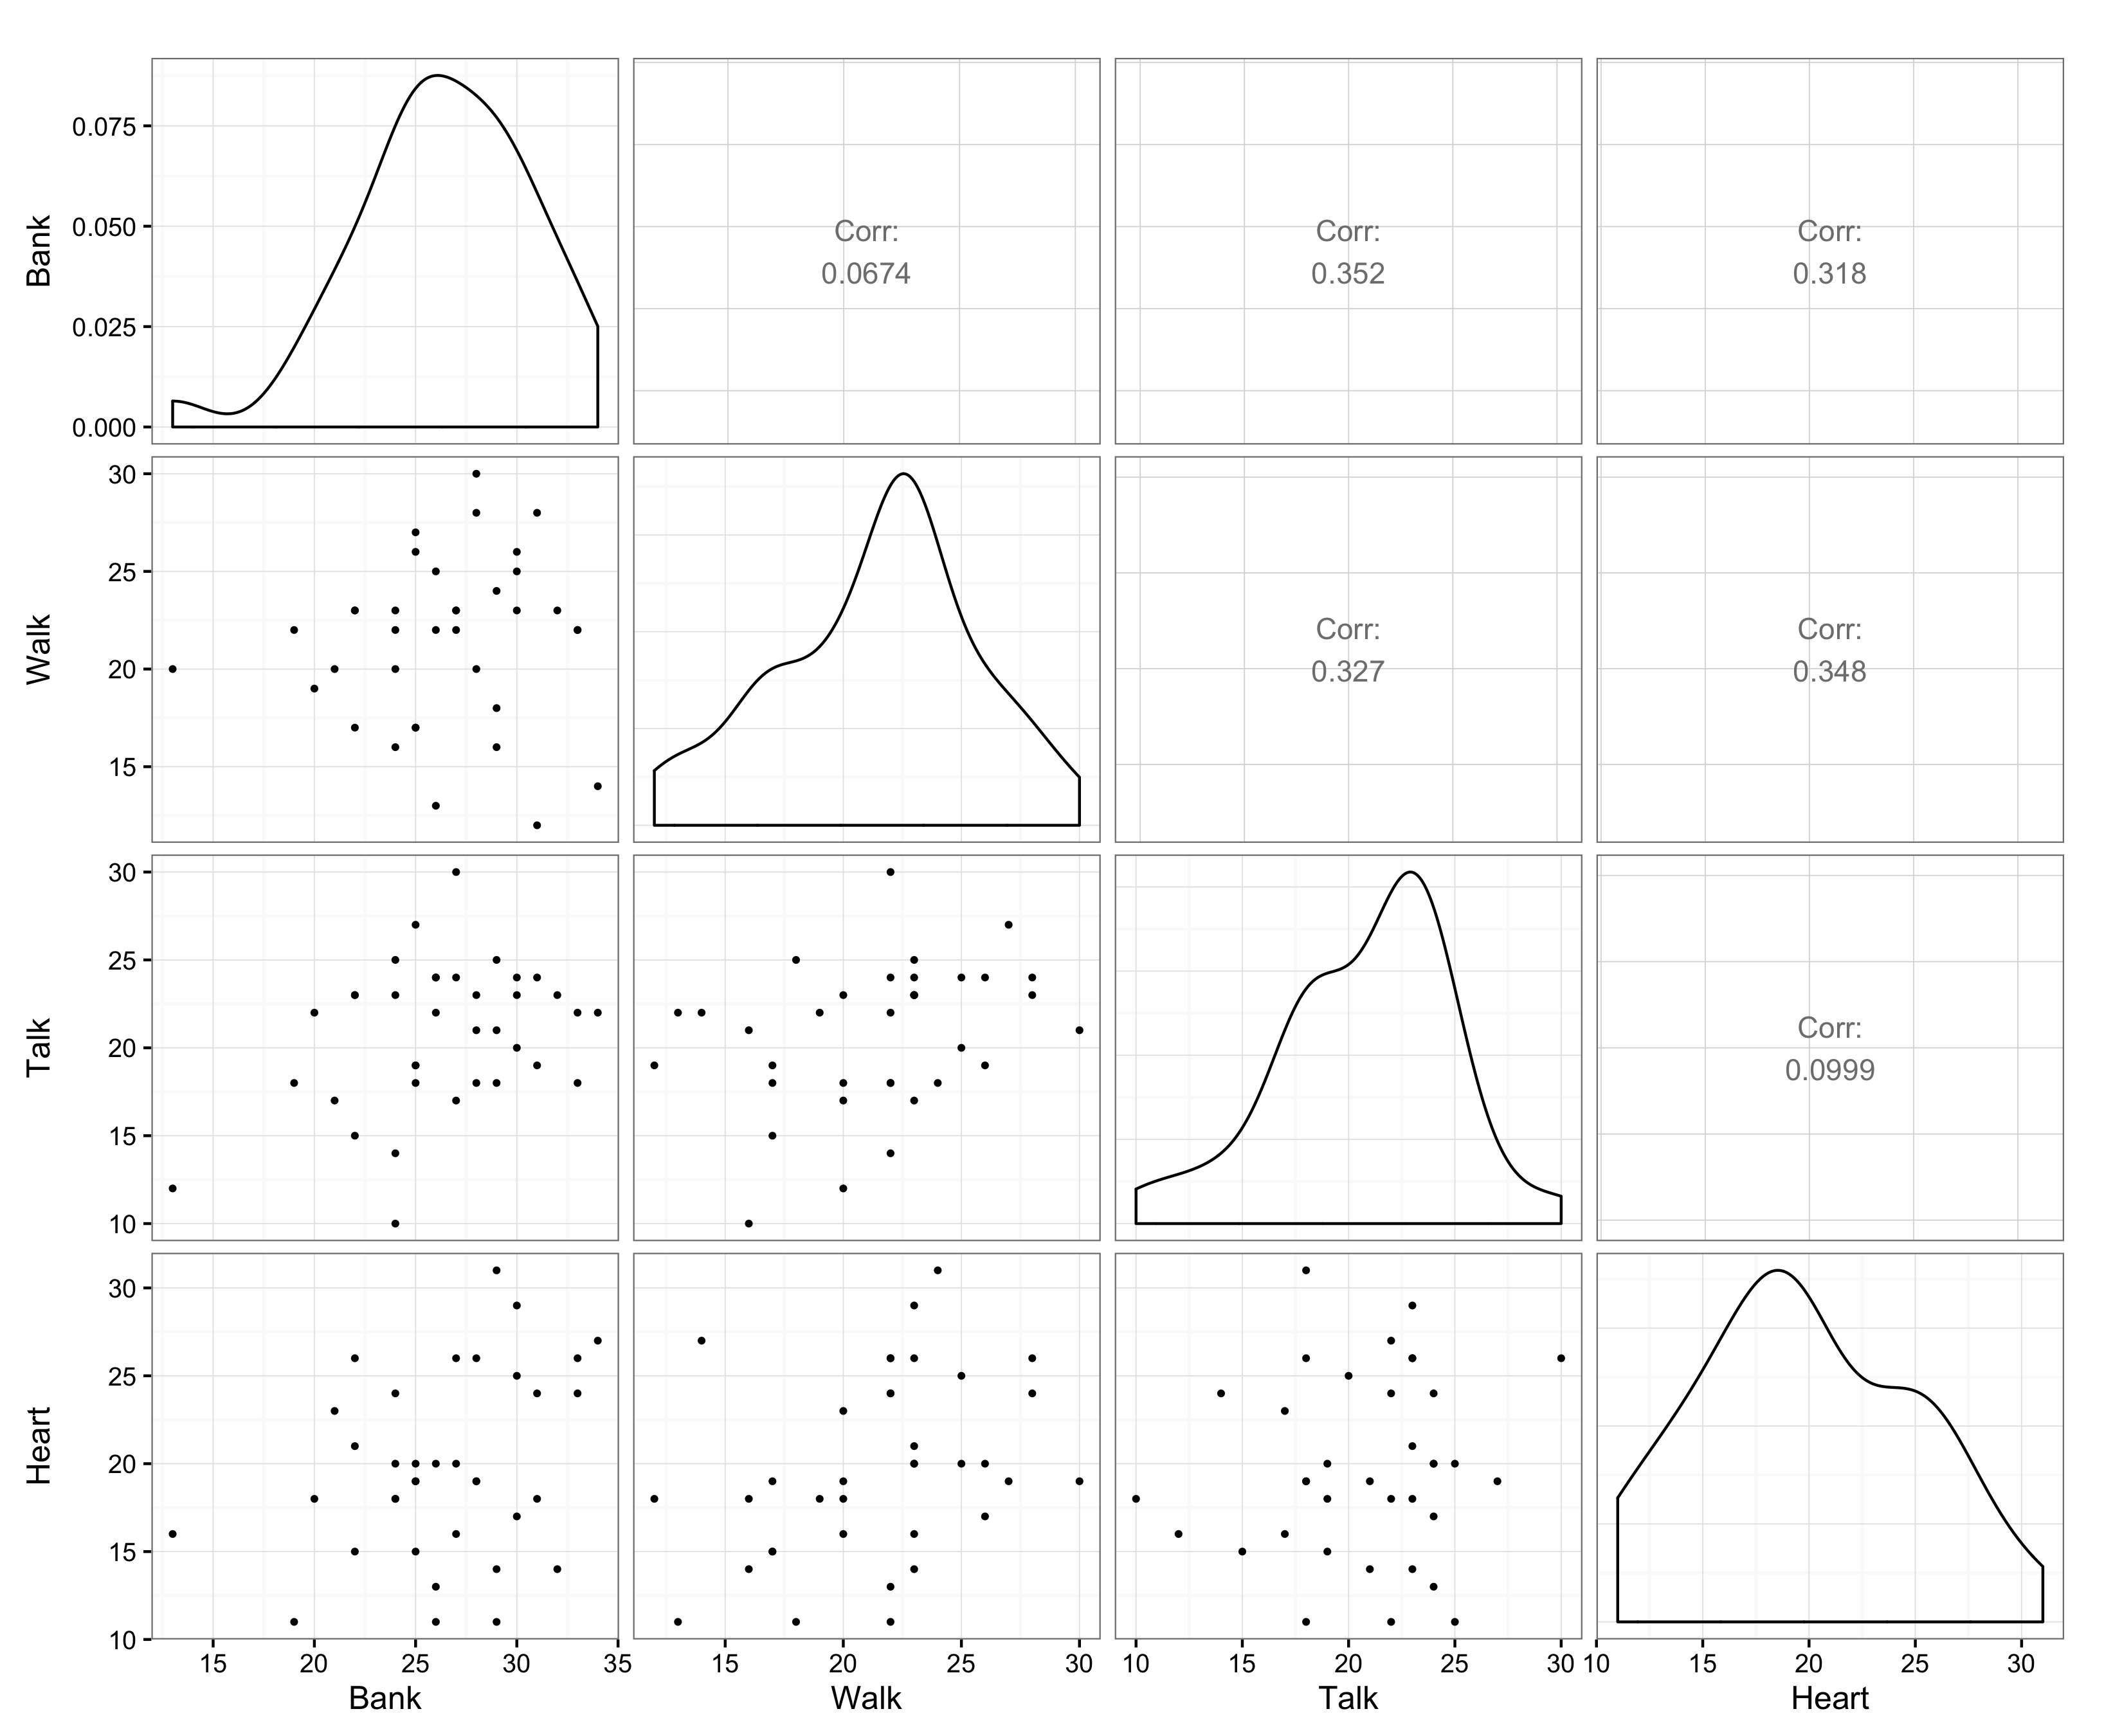
\includegraphics[width=\textwidth]{1a.png}
	\caption{Pairwise scatterplots of the variables in the ``Pace of Life and Heart Disease'' dataset.}
	\label{fig:1a}
\end{figure}

\part \textit{Obtain the least squares fit to the linear regression of heart on bank, walk, and talk.} \label{prob:0914b}

\begin{codeSmall}
> lm1 <- lm(Heart ~ Bank + Walk + Talk, data=paceData)
> summary(lm1)

Call:
lm(formula = Heart ~ Bank + Walk + Talk, data = paceData)

Residuals:
    Min      1Q  Median      3Q     Max 
-8.4014 -3.0263  0.0602  2.6748  8.4646 

Coefficients:
            Estimate Std. Error t value Pr(>|t|)  
(Intercept)   3.1787     6.3369   0.502   0.6194  
Bank          0.4052     0.1971   2.056   0.0480 *
Walk          0.4516     0.2009   2.248   0.0316 *
Talk         -0.1796     0.2222  -0.808   0.4249  
---
Signif. codes:  0 ‘***’ 0.001 ‘**’ 0.01 ‘*’ 0.05 ‘.’ 0.1 ‘ ’ 1

Residual standard error: 4.805 on 32 degrees of freedom
Multiple R-squared:  0.2236,	Adjusted R-squared:  0.1509 
F-statistic: 3.073 on 3 and 32 DF,  p-value: 0.04162
\end{codeSmall}

\part \textit{Plot the residuals versus the fitted values. Is there evidence that the variance of the residuals increases with increasing fitted values or that there are any outliers?}

The residual plot is shown in Figure \ref{fig:1c}. There does not seem to be evidence that the variance of the residuals increases with increasing fitted values, or that there are any extreme outliers.

\begin{figure}[!h]
	\centering
	\captionsetup{width=0.8\textwidth}
	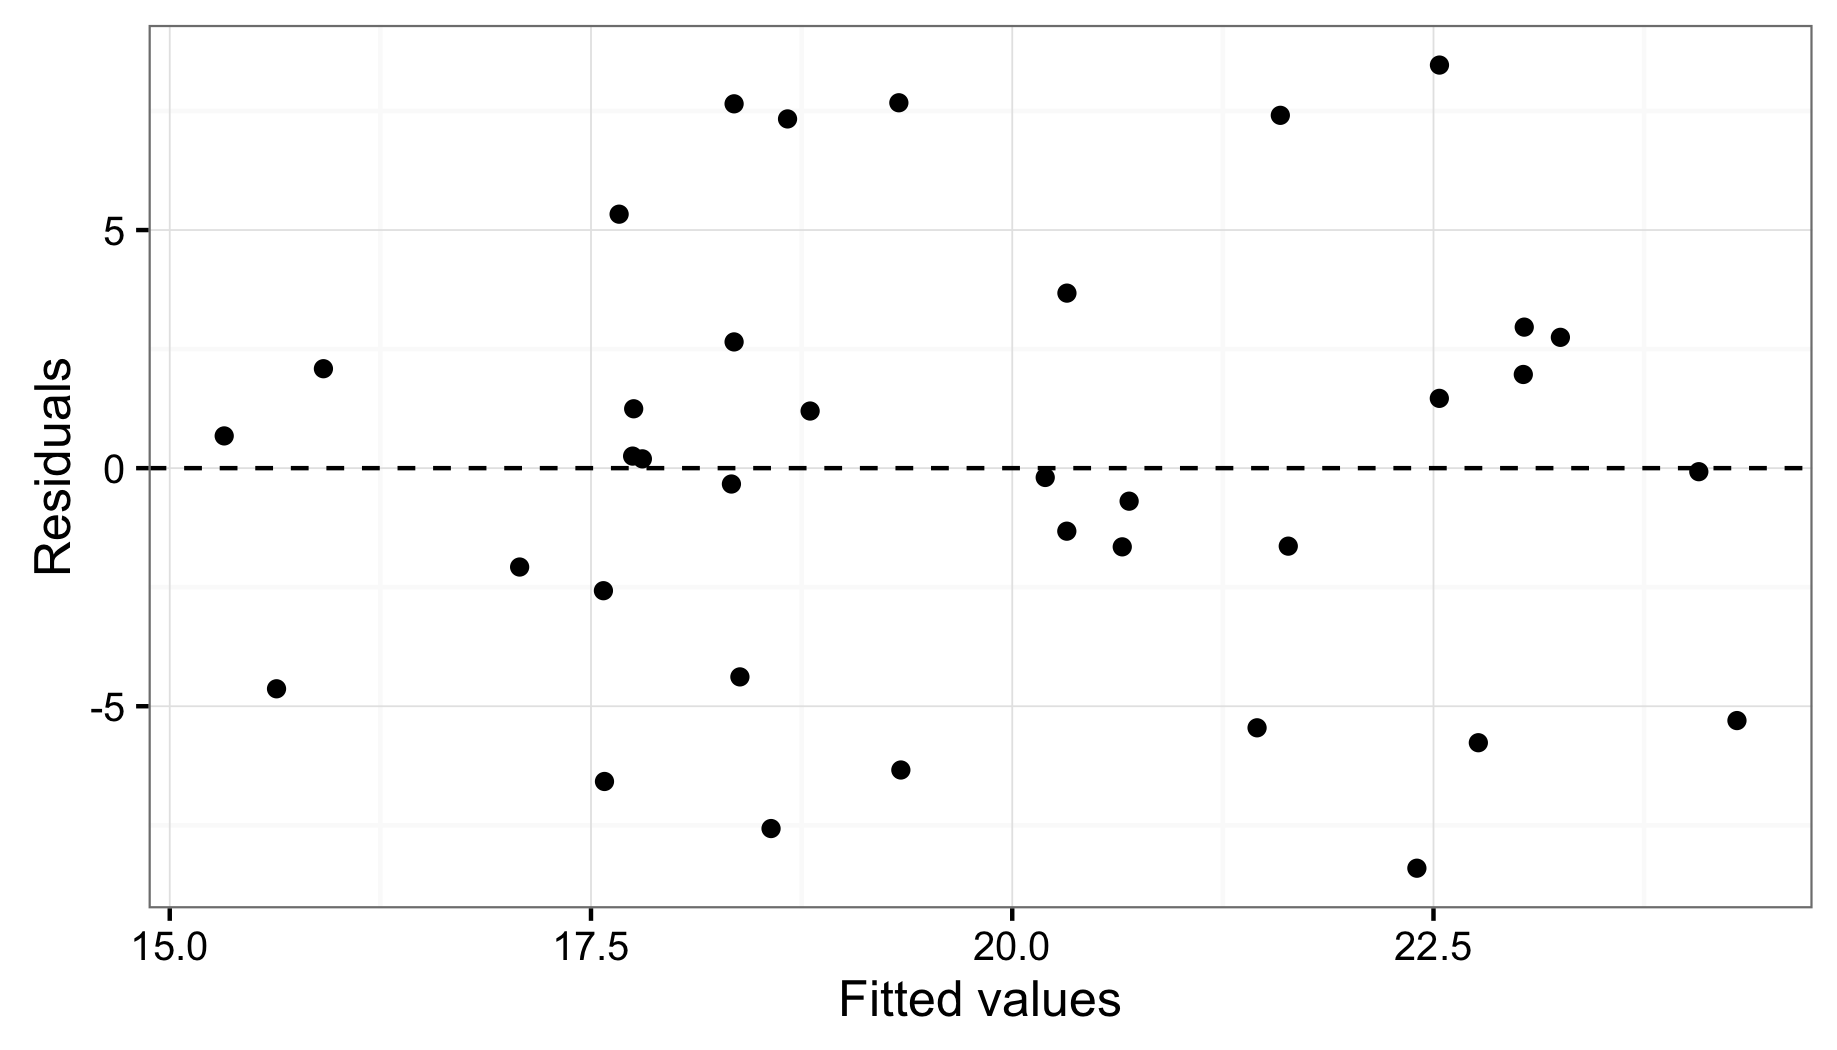
\includegraphics[width=4.25in]{1c.png}
	\caption{Residual plot for the fitted model from part (\ref{prob:0914b}).}
	\label{fig:1c}
\end{figure}

\part \textit{Report a summary of the least squares fit. Write down the estimated equation with standard errors below each estimated coefficient.}

Under the parallel lines regression model, the age-adjusted death rate due to heart disease (\texttt{Heart}) increases by $0.4052$ for every one unit increase in the bank clerk speed (\texttt{Bank}) (95\% confidence interval from $0.0037$ to $0.8067$). Similarly, \texttt{Heart} increases by $.4516$ for every one unit increase in the pedestrian walking speed (\texttt{Walk}) (95\% confidence interval from $0.0424$ to $0.8608$). The data provides no evidence that \texttt{Heart} is associated with postal clerk talking speed (\texttt{Talk}) (two sided p-value = $0.4249$ for a test that the \texttt{Talk} coefficient is zero).



\end{parts}


\titledquestion{\ramsey 9.16}




\titledquestion{\ramsey 9.18}




\titledquestion{\ramsey 9.20}




\titledquestion{\ramsey 10.19}




\titledquestion{\ramsey 10.28}




\end{questions}

%\listoftodos

\end{document}